% GGS 662 Assignment 3 -- research proposal deck (5-minute talk).
% Build (from this folder), run twice:
%   pdflatex -interaction=nonstopmode -output-directory=.build assignment3_proposal.tex && cp .build/assignment3_proposal.pdf .
% Content sources: ../lab_inputs.ipynb (A3, L1, H1-H6) and ../outputs/*.md (agent stages).
% Red TODOs must be resolved before submitting.
\documentclass[aspectratio=169,11pt]{beamer}
% ---- "Panchromatic" theme: graphite on film grey, one radar-cyan accent, IBM Plex,
% ---- a mono kicker above each title and a map scale-bar rule under it.
\usetheme{default}
\usepackage[T1]{fontenc}
\usepackage[sfdefault,scale=0.92]{plex-sans}
\usepackage[scale=0.86]{plex-mono}
\usepackage{appendixnumberbeamer}
\usepackage{booktabs}
\usepackage{colortbl}
\usepackage{tabularx}
\usepackage{array}
\usepackage{tikz}
\usetikzlibrary{positioning,arrows.meta,calc,fadings}

\definecolor{navy}{HTML}{15181B}      % graphite (headings, dark panels)
\definecolor{ink}{HTML}{23272B}
\definecolor{muted}{HTML}{6E7378}
\definecolor{teal}{HTML}{127C8E}      % radar cyan accent
\definecolor{tealtint}{HTML}{E3EEF0}
\definecolor{amber}{HTML}{B4520F}     % used sparingly for emphasis
\definecolor{ambertint}{HTML}{F5EBE2}
\definecolor{failred}{HTML}{A12A1F}
\definecolor{paper}{HTML}{F3F2EE}     % film grey
\definecolor{rule}{HTML}{CFCBC2}
\definecolor{panel}{HTML}{FAF9F6}

\setbeamertemplate{navigation symbols}{}
\setbeamercolor{normal text}{fg=ink,bg=paper}
\setbeamercolor{background canvas}{bg=paper}
\setbeamercolor{structure}{fg=teal}
\setbeamercolor{alerted text}{fg=amber}
\setbeamercolor{block title}{bg=rule!55,fg=navy}
\setbeamercolor{block body}{bg=panel,fg=ink}
\setbeamertemplate{blocks}[default]
\setbeamerfont{block title}{series=\bfseries,size=\small}
\setbeamerfont{frametitle}{size=\Large,series=\bfseries}
\setbeamerfont{framesubtitle}{family=\ttfamily,size=\scriptsize}
\setbeamertemplate{itemize item}{\textcolor{teal}{\rule[0.25ex]{0.9ex}{0.9ex}}}
\setbeamertemplate{itemize subitem}{\textcolor{muted}{\rule[0.35ex]{0.6ex}{0.6ex}}}
\setbeamertemplate{enumerate item}{\textcolor{teal}{\ttfamily\footnotesize\insertenumlabel}}
\setlength{\leftmargini}{1.1em}

% kicker (frame subtitle) + title + scale-bar rule
\makeatletter
\setbeamertemplate{frametitle}{%
  \vspace*{0.55cm}%
  \ifx\insertframesubtitle\@empty\else{\usebeamerfont{framesubtitle}\color{teal}\MakeUppercase{\insertframesubtitle}}\par\vspace{1pt}\fi
  {\usebeamerfont{frametitle}\color{navy}\insertframetitle}\par\vspace{4pt}%
  
\begin{tikzpicture}
    \foreach \i in {0,1,2,3}{\pgfmathsetmacro{\c}{mod(\i,2)==0?"navy":"paper"}
      \draw[navy,line width=0.3pt,fill=\c] (\i*0.55,0) rectangle ++(0.55,0.09);}
    \draw[rule,line width=0.5pt] (2.3,0.045) -- (\textwidth-0.2cm,0.045);
  \end{tikzpicture}\par\vspace{2pt}}
\makeatother

\setbeamertemplate{footline}{%
  \hbox to \paperwidth{\hspace{0.9cm}{\color{rule}\leaders\hrule height 0.4pt\hfill}\hspace{0.9cm}}\vspace{3pt}
  \hbox to \paperwidth{\hspace{0.9cm}{\ttfamily\tiny\color{muted}GGS 662 \enskip/\enskip ASSIGNMENT 3 \enskip/\enskip J.\,ROGERS}\hfill
  {\ttfamily\tiny\color{muted}\ifnum\insertframenumber<10 0\fi\insertframenumber\,/\,\inserttotalframenumber}\hspace{0.9cm}}\vspace{7pt}}
\setbeamersize{text margin left=0.9cm,text margin right=0.9cm}

% faint graticule for dark panels
\newcommand{\graticule}{%
  \foreach \x in {0,1.6,...,16.4} \draw[white,opacity=0.06,line width=0.4pt] ([xshift=\x cm]current page.south west) -- ([xshift=\x cm]current page.north west);
  \foreach \y in {0,1.6,...,9.6} \draw[white,opacity=0.06,line width=0.4pt] ([yshift=\y cm]current page.south west) -- ([yshift=\y cm]current page.south east);}

\newcommand{\todo}[1]{\textcolor{red}{\textbf{TODO: #1}}}
\newcommand{\acc}{\textcolor{teal}{\textbf{Accepted}}}
\newcommand{\chg}{\textcolor{amber}{\textbf{Changed}}}
\newcommand{\rej}{\textcolor{failred}{\textbf{Rejected}}}
\newcolumntype{Y}{>{\raggedright\arraybackslash}X}

\title{What does an agent add?}
\author{Justin Rogers}
\date{October 5, 2026}

\begin{document}

% ------------------------------------------------------------------ 1
\begin{frame}[plain]
\begin{tikzpicture}[remember picture,overlay]
  \fill[navy] (current page.south west) rectangle (current page.north east);
  \IfFileExists{images/title_pan.jpg}{%
    \node[anchor=east,inner sep=0] at (current page.east) {\includegraphics[height=\paperheight]{images/title_pan.jpg}};
    \fill[navy,opacity=0.35] (current page.south west) rectangle (current page.north east);
    \fill[navy,opacity=0.93] (current page.south west) rectangle ([xshift=8.4cm]current page.north west);
    \fill[navy,path fading=east,opacity=0.93] ([xshift=8.4cm]current page.south west) rectangle ([xshift=11.4cm]current page.north west);
  }{\graticule}
  \node[anchor=north west,text=teal!70!white,font=\ttfamily\footnotesize] at ([xshift=0.9cm,yshift=-1.0cm]current page.north west) {RESEARCH PROPOSAL \enskip/\enskip GGS 662 ASSIGNMENT 3};
  \node[anchor=north west,text width=7.2cm,text=paper,align=left] at ([xshift=0.9cm,yshift=-1.6cm]current page.north west)
    {{\fontsize{30}{33}\selectfont\bfseries What does an agent add?}};
  \foreach \i in {0,1,2,3}{\pgfmathsetmacro{\c}{mod(\i,2)==0?"paper":"navy"}
    \draw[paper,line width=0.3pt,fill=\c] ([xshift=0.9cm+\i*0.55cm,yshift=-4.25cm]current page.north west) rectangle ++(0.55,0.09);}
  \node[anchor=north west,text width=7.0cm,text=paper!80,align=left] at ([xshift=0.9cm,yshift=-4.55cm]current page.north west)
    {\small Comparing a tool-grounded LLM agent with a vision-language model and non-agent baselines for new-building detection in Sentinel-1 SAR and Landsat panchromatic time series};
  \node[anchor=south west,text width=7.2cm,text=paper!70,align=left,font=\small] at ([xshift=0.9cm,yshift=0.8cm]current page.south west)
    {\textbf{Justin Rogers}\\ {\ttfamily\scriptsize GEORGE MASON UNIVERSITY \enskip/\enskip OCTOBER 5, 2026}};
  \IfFileExists{images/title_pan.jpg}{\node[anchor=south east,text=paper!75,font=\ttfamily\tiny,fill=navy,fill opacity=0.6,text opacity=1] at ([xshift=-0.3cm,yshift=0.3cm]current page.south east) {London and the Thames, Landsat 7, 2002 (shown in greyscale). NASA Earth Observatory / R. Simmon, USGS data. Public domain};}{}
\end{tikzpicture}
\note{About 15 s. Topic: can an AI agent help interpret large satellite archives over time, and what does the agent itself add?}
\end{frame}

% ------------------------------------------------------------------ 2
\begin{frame}[shrink=22]{The problem: large image archives, unreliable AI interpreters}{01 / Problem}
\begin{columns}[T,onlytextwidth]
\column{0.55\textwidth}
\begin{itemize}
  \item Satellite archives now hold years of monthly SAR and optical images per place. Reading change from them by hand does not scale.
  \item Current multimodal models are weak at this:
  \begin{itemize}
    \item best of 18 models: 34.1\% \textbf{accuracy} (share of city-change benchmark questions answered correctly) (Xuan et al., 2025)
    \item LLM agents on yes/no Earth-observation questions: 40\% \textbf{accuracy} zero-shot, about 60\% with self-reflection, where guessing scores 50\%; generated code \textbf{failed to run} in over 44\% of runs (Kao et al., 2026)
    \item TEOChat, a temporal vision-language model, handles at most 8 images per sequence (Irvin et al., 2025)
  \end{itemize}
  \item Tool-using agents are the promising route (Feng et al., 2026), but SAR and panchromatic data are rarely tested.
\end{itemize}
\column{0.40\textwidth}
\includegraphics[width=\linewidth]{images/urban_growth.jpg}\\[-2pt]
{\ttfamily\tiny\color{muted} Las Vegas 1999 vs 2024 (Landsat 7, USGS; public domain)}
\vspace{4pt}
\begin{block}{What this study tests}
\small Whether grounding an LLM in sensor tools makes it \alert{more accurate and less prone to fabrication} than a VLM reading the same imagery, and what its reasoning adds over non-agent rules given the same tool outputs.
\end{block}
\end{columns}
\note{About 35 s. Numbers are from the reviewed papers. Gap is worded as "not found in our search".}
\end{frame}

% ------------------------------------------------------------------ 3
\begin{frame}{How I used the multi-agent workflow}{02 / Workflow}
\centering
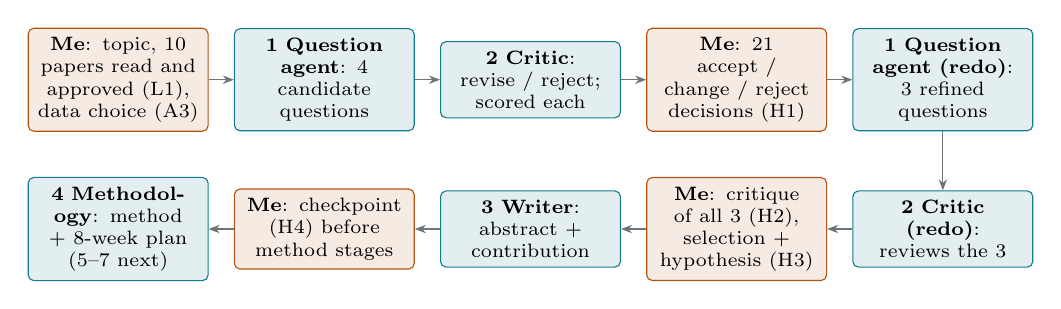
\begin{tikzpicture}[
  ag/.style={draw=teal,fill=tealtint,rounded corners=2pt,minimum height=0.85cm,text width=2.05cm,align=center,font=\scriptsize},
  me/.style={draw=amber,fill=ambertint,rounded corners=2pt,minimum height=0.85cm,text width=2.05cm,align=center,font=\scriptsize},
  ar/.style={-{Stealth[length=4pt]},color=muted},
  node distance=0.32cm]
\node[me] (a) {\textbf{Me}: topic, 10 papers read and approved (L1), data choice (A3)};
\node[ag,right=of a] (b) {\textbf{1 Question agent}: 4 candidate questions};
\node[ag,right=of b] (c) {\textbf{2 Critic}: revise / reject; scored each};
\node[me,right=of c] (d) {\textbf{Me}: 21 accept / change / reject decisions (H1)};
\node[ag,right=of d] (e) {\textbf{1 Question agent (redo)}: 3 refined questions};
\node[ag,below=0.75cm of e] (f) {\textbf{2 Critic (redo)}: reviews the 3};
\node[me,left=of f] (g) {\textbf{Me}: critique of all 3 (H2), selection + hypothesis (H3)};
\node[ag,left=of g] (h) {\textbf{3 Writer}: abstract + contribution};
\node[me,left=of h] (i) {\textbf{Me}: checkpoint (H4) before method stages};
\node[ag,left=of i] (j) {\textbf{4 Methodology}: method + 8-week plan (5--7 next)};
\foreach \x/\y in {a/b,b/c,c/d,d/e,e/f,f/g,g/h,h/i,i/j} \draw[ar] (\x) -- (\y);
\end{tikzpicture}

\vspace{8pt}
{\small \textcolor{amber}{\rule{8pt}{8pt}} human decision \qquad \textcolor{teal}{\rule{8pt}{8pt}} agent stage (fresh agent, given only a prompt packet) \qquad every output and packet archived}
\note{About 30 s. Each agent gets a self-contained packet built from my form; I decide at every orange box. Agreement between agents is not treated as validation.}
\end{frame}

% ------------------------------------------------------------------ 4
\begin{frame}[shrink=14]{Three refined questions and my critique}{03 / Questions}
\scriptsize
\begin{tabularx}{\textwidth}{@{}>{\raggedright\arraybackslash}p{3.4cm}YY>{\raggedright\arraybackslash}p{2.9cm}@{}}
\toprule
\textbf{Question} {\color{muted}(origin)} & \textbf{Scientific value (my critique)} & \textbf{Feasibility in 8 weeks (my critique)} & \textbf{Outcome} \\
\midrule
\textbf{Q1.} Is a tool-using agent \emph{no worse} than a fixed pipeline with the same tools, better where the tools disagree, and does it abstain when data are missing? {\color{muted}(AI, edited by me)}
 & Strong comparison. It is detection, not description, but tool outputs from classic CV methods act as extra features instead of the model interpreting from scratch.
 & Feasible at test level; a production system across many areas would take longer.
 & \textcolor{teal}{\textbf{Selected}}, then reshaped by me: VLM comparison added, identical inputs \\
\addlinespace
\textbf{Q2.} Does panchromatic imagery (15\,m resolution) add anything to Sentinel-1 SAR? {\color{muted}(AI, edited by me)}
 & Good idea, but I would flip it: \alert{panchromatic supported by SAR}, since panchromatic is more common in commercial imagery.
 & Hard from scratch in 8 weeks; possible with an AI expert or by building on prior research.
 & \textcolor{amber}{\textbf{Kept inside Q1}} as a secondary analysis, flipped to panchromatic-led \\
\addlinespace
\textbf{Q3.} Does neighbouring-cell context help the agent place change in the right cell? {\color{muted}(AI)}
 & Reasonable, but too general: extra context could be almost anything, and it has no target problem.
 & Feasible.
 & \textcolor{muted}{\textbf{Deferred}} to follow-on work (not rejected) \\
\bottomrule
\end{tabularx}
\note{About 40 s. These critiques are mine. They decided the outcome column: Q1 selected and reshaped, Q2 folded in and flipped, Q3 parked as future work.}
\end{frame}

% ------------------------------------------------------------------ 5
\begin{frame}[shrink=16]{From three questions to one: Q1, reshaped by my critique}{04 / Selection}
\begin{block}{Research question}\small
In held-out SpaceNet 7 areas (2017--2020), does an LLM agent with built-in SAR and panchromatic tools detect new buildings (presence and month) in 100\,m cells more accurately than \alert{a vision-language model that looks at the imagery directly}, and than \alert{non-agent baselines given the same tool outputs}? Does it fabricate fewer answers?
\end{block}
\begin{columns}[T,onlytextwidth]
\column{0.48\textwidth}
\textbf{How the three critiques shaped it}
\begin{itemize}\footnotesize
  \item \textbf{Q1} isolates what the agent adds (same tools); I added the VLM comparison, my core interest.
  \item \textbf{Q2} lives on inside it: panchromatic-only vs panchromatic + SAR, led by panchromatic as I suggested.
  \item \textbf{Q3} is deferred: reasonable and feasible, but too general for 8 weeks.
\end{itemize}
\column{0.48\textwidth}
\textbf{Hypothesis}
\begin{itemize}\footnotesize
  \item Tool grounding reduces hallucination: the agent is more accurate than the VLM and fabricates fewer answers.
  \item Against a tuned rule and a fitted rule on the same tool outputs, the agent is at least as accurate (difference with a confidence interval) and better where the tools disagree.
\end{itemize}
\end{columns}
\vspace{2pt}{\scriptsize\color{muted} Same inputs for both: the same 1\,km chips (pan 15\,m, SAR 10\,m resolution), the same 8 dates, the same question.}
\note{About 35 s. Transition: my critique did not just pick a winner. Q1 absorbed Q2 and was reshaped by my VLM decision; Q3 is parked. The same-tool baselines show whether the agent's reasoning is what helps.}
\end{frame}

% ------------------------------------------------------------------ 6
\begin{frame}[shrink=10]{AI suggestions I accepted, changed or rejected}{05 / Critical review}
\footnotesize
\begin{tabularx}{\textwidth}{@{}p{4.6cm}p{1.6cm}Y@{}}
\toprule
\textbf{AI suggestion} & \textbf{Decision} & \textbf{Why} \\
\midrule
Critic: an agent-vs-VLM comparison is confounded; first log dropped the VLM & \chg & \textbf{Reinstated by me}: it is my core question. Made fair with 1\,km chips and the VLM's full frame limit, and paired with same-tool baselines. \\
Hand-label 300--500 cells; use NAIP for dates & \rej & SpaceNet 7 already has monthly building labels from separate imagery; saves about two weeks. \\
Critic: add a fitted baseline; replace the margin $\delta$ with confidence intervals & \acc & A second baseline on the same tool outputs; intervals instead of an arbitrary margin. \\
Critic's revised question: agent vs fixed pipeline & \acc & The only contrast that isolates what the agent adds. \\
Panchromatic as an optional ablation & \chg & Required secondary analysis, and panchromatic-led (my Q2 critique). \\
Single area split into blocks & \chg & Whole areas held out (AOI-level split): less leakage, better external validity. \\
Critic: reject the neighbourhood question (Q3) & \chg & Not rejected, just not selected: reasonable and feasible, but too general for this paper; kept as a follow-on. \\
\bottomrule
\end{tabularx}
\vspace{3pt}{\scriptsize\color{muted} Full log: 21 decisions (form field H1); earlier outputs and every agent's input packet are archived.}
\note{About 35 s. This is the critical-review evidence: what I kept, changed and threw out, and why.}
\end{frame}

% ------------------------------------------------------------------ 7
\begin{frame}[shrink=22]{Literature and contribution}{06 / Literature}
\footnotesize
\begin{tabularx}{\textwidth}{@{}p{3.6cm}YY@{}}
\toprule
\textbf{Paper} & \textbf{What it established} & \textbf{What this work adds} \\
\midrule
Kao et al. (2026), ACL Findings & LLM agents reach about 60\% accuracy at best on yes/no EO questions (guessing: 50\%); generated code often fails to run & Predefined, deterministic tools instead of free-form code \\
Feng et al. (2026), ICLR & Tool-using EO agent (Earth-Agent, 104 tools) & A SAR + panchromatic tool set and a same-tools baseline \\
Xuan et al. (2025), NeurIPS & Best of 18 multimodal models: 34.1\% accuracy (questions answered correctly) on a city-change benchmark & Grounds answers in time-series statistics \\
Lee et al. (2026), IEEE JSTARS & SAR time-series change types; up-steps linked to construction & Uses the SAR change test inside an agent \\
Qu et al. (2026), Remote Sens. Environ. & Dense time-series change detection; AOI-level split; misalignment creates false change & Same split logic and misregistration checks \\
Zuo et al. (2026), IEEE JSTARS & Hallucinated change is a known failure; change-vector-analysis calibration plus self-consistency reduces it & Measures abstention and fabricated answers \\
\bottomrule
\end{tabularx}
\vspace{3pt}
{\footnotesize\textbf{Proposed contribution:} a controlled comparison of a tool-grounded LLM agent with a vision-language model and with same-tool baselines, on a dense SAR + panchromatic archive, scored against independent monthly labels. \alert{Proposed, not established.}}
\note{About 30 s. All 10 references read and verified; full list in the supporting slides.}
\end{frame}

% ------------------------------------------------------------------ 8
\begin{frame}[shrink=26]{Data and method}{07 / Method}
\begin{columns}[T,onlytextwidth]
\column{0.47\textwidth}
\textbf{\small Data (all public)}
\begin{itemize}\footnotesize
  \item \textbf{Panchromatic:} Landsat-8 band 8 at 15\,m resolution (each pixel covers 15\,$\times$\,15\,m of ground), monthly, already co-registered (MuRA-T, 60 SpaceNet 7 areas, 2017--2020)
  \item \textbf{SAR:} Sentinel-1 C-band GRD, one orbit track per area, co-registered by me
  \item \textbf{Reference:} SpaceNet 7 monthly building footprints, traced on separate PlanetScope imagery
  \item \textbf{Unit:} 100\,m cells in 10--20 areas; whole areas held out for testing
\end{itemize}
\column{0.49\textwidth}
\textbf{\small Steps}
\begin{enumerate}\footnotesize
  \item Build tools: SAR change test, panchromatic change magnitude, pretrained CNN change detector, data availability
  \item \textbf{Tuned baseline:} fixed rule on the same tools, tuned on development areas
  \item \textbf{Agent:} same tools, answers \texttt{presence / onset month / abstain}
  \item \textbf{VLM:} reads the same 1\,km chips on the same 8 dates as the agent's tools
  \item \textbf{Fitted baseline:} simple classifier on the same tool outputs
  \item Controls: same LLM without tools; pan-only vs pan + SAR (pipeline)
  \item Freeze, pre-register, run test areas once
\end{enumerate}
{\footnotesize\textbf{AI-assisted coding:} Claude Code writes the data, tool and analysis code; I review every function and test it on synthetic images with known change. No LLM scores answers.}
\end{columns}
\note{About 35 s. No model training. The baseline uses exactly the agent's tools.}
\end{frame}

% ------------------------------------------------------------------ 9
\begin{frame}{What we validate, and how}{08 / Validation}
\vspace{-6pt}
\footnotesize
\renewcommand{\arraystretch}{1.35}
\resizebox{\linewidth}{!}{\begin{tabular}{@{}>{\raggedright\arraybackslash}p{4.2cm}>{\raggedright\arraybackslash}p{9.6cm}>{\raggedright\arraybackslash}p{5.6cm}@{}}
\toprule
\textbf{What is validated} & \textbf{How} & \textbf{Fails if} \\
\midrule
\textbf{1. The reference labels} & Traced on separate PlanetScope imagery; label lag measured & Lag swamps onset error \\
\textbf{2. The tools} & Tested alone on development areas and on synthetic known change & Tool F1 near chance \\
\textbf{3. A fair comparison} & Same chips, dates and question logged for agent and VLM & Any input mismatch \\
\textbf{4. Evidence, not memory} & Opaque cell IDs; same LLM with tools disabled & No-tools accuracy near the agent's \\
\textbf{5. The agent uses its tools} & Tool evidence shuffled between cells & Accuracy barely drops \\
\textbf{6. Less hallucination} & Unanswerable queries; cited values checked against tool logs & Fabricates as often as the VLM \\
\textbf{7. Generalises to new areas} & Whole areas held out; area-level confidence intervals & Agent $-$ VLM interval includes zero \\
\textbf{8. Robustness} & One-pixel shift, 200\,m cells, SAR look direction; 3 repeat runs & Result flips \\
\bottomrule
\end{tabular}}

\vspace{2pt}
{\scriptsize\textbf{Metrics:} F1 score (balance of precision and recall), precision, recall, onset error in months, fabrication rate (answers given when the correct answer is ``abstain''); deterministic scoring, no LLM judge.\par
\textbf{Spatial assumptions:} sub-pixel co-registration; cells measured in metres; labels mark visible buildings, so SAR change should lead them. \textbf{Key risks:} sparse Sentinel-1 scenes in some areas; weak tools at 15\,m resolution; VLM setup time; API budget.\par}
\note{About 40 s. Each row is one thing we validate and how it could fail. Name the main falsifier: if the confidence interval for agent minus VLM includes zero, the hypothesis fails.}
\end{frame}

% ------------------------------------------------------------------ 10
\begin{frame}[shrink=10]{Eight-week plan, journal and co-authors}{09 / Plan}
\begin{columns}[T,onlytextwidth]
\column{0.44\textwidth}
\scriptsize
\begin{tabular}{@{}lp{5.6cm}@{}}
\toprule
\textbf{Week} & \textbf{Work} \\
\midrule
1 & Download data; choose areas, VLM and CNN; draft pre-registration \\
2 & Grid, labels, 1\,km chips; validate each tool on its own \\
3 & Agent and VLM harness; tune and fit baselines; pilot \\
4 & Freeze, pre-register; run all arms on test areas \\
5 & Score; area-level confidence intervals; robustness \\
6 & Draft paper \\
7 & Co-author and critic review; check claims; revise \\
8 & Final checks; package code and data; submit \\
\bottomrule
\end{tabular}
\column{0.53\textwidth}
{\footnotesize\textbf{Journal:} \emph{International Journal of Applied Earth Observation and Geoinformation} (Elsevier, open access). \textbf{2025 JIF 8.2}, Q1 in Remote Sensing (7/66); source: Clarivate Journal Citation Reports, 2025 JCR year (June 2026 release). Publishes applied EO methods, SAR and building change detection, and GeoAI, which fits an agent-vs-VLM evaluation on SAR + panchromatic time series.}
\vspace{6pt}
\textbf{Possible co-authors} {\scriptsize(neither has agreed)}
\begin{itemize}\scriptsize
  \item \textbf{Dr.\ Edward Oughton}, GMU Geography \& Geoinformation Science: agentic GeoAI and spatial computing. Checks: workflow design, evaluation protocol, reproducibility.
  \item \textbf{Dr.\ Konrad Wessels}, GMU Geography \& Geoinformation Science: SAR and time-series remote sensing. Checks: SAR preprocessing, co-registration, physical plausibility of SAR change.
\end{itemize}
\end{columns}
\note{About 30 s. Plan detail is in the supporting slides.}
\end{frame}

% ------------------------------------------------------------------ 11
\begin{frame}[shrink=18]{Sources and AI disclaimer}{10 / Sources}
\footnotesize
\textbf{Data:} MuRA-T (Purdue RVL; Deshmukh et al., 2023, arXiv:2302.12301, GPL v3); SpaceNet 7 (Van Etten et al., CVPR 2021, CC BY-SA 4.0); Copernicus Sentinel-1 (ESA); Landsat-8 (USGS). \textbf{Images:} title, NASA Earth Observatory image by Robert Simmon using USGS Landsat data (public domain, shown in greyscale); slide 2, USGS Landsat Missions, Las Vegas 1999--2024 (public domain). Full references: supporting slides.

\vspace{6pt}
\textbf{AI tools and what they did:} Claude Code (Anthropic, Claude Opus 5.5) built the orchestration script and prompt packets; ran the question, critic, writer and methodology roles as fresh agents (methodology-critic, data + tools and validation roles not run before submission); searched the literature, downloaded the full papers and checked every cited claim against them; found the MuRA-T dataset and openly licensed images; checked the journal metric (the first choice, IJDE, was on hold, so the target became JAG); drafted the first decision-log rows and data notes at my direction; and generated these slides.

\vspace{4pt}
\textbf{Resources used:} Crossref (DOI checks); arXiv, CVF Open Access and publisher PDFs (full papers); Clarivate Journal Citation Reports (journal metric); NASA Earth Observatory and USGS Landsat galleries (images); Purdue RVL and AWS Open Data (datasets).

\vspace{6pt}
\textbf{My own checks:} read and approved all 10 references; wrote my own critique of the three questions; selected the question and hypothesis; chose the co-authors; added my own decision-log rows after the critic's review, including reinstating the VLM comparison. Agreement between agents was not treated as validation.
\note{About 15 s.}
\end{frame}

% ------------------------------------------------------------------ 12
\begin{frame}[plain]
\begin{tikzpicture}[remember picture,overlay]
  \fill[navy] (current page.south west) rectangle (current page.north east); \graticule
  \node[text=paper,align=center] at (current page.center) {{\fontsize{30}{34}\selectfont\bfseries Questions?}\\[10pt]{\ttfamily\small\color{teal!70!white} WHAT DOES THE AGENT ADD THAT THE SAME TOOLS DO NOT?}};
\end{tikzpicture}
\end{frame}

\appendix
% ------------------------------------------------------------------ S1
\begin{frame}[shrink=8]{References (APA 7), 1 of 2}{Supporting}
\scriptsize
\begin{itemize}
\item Deshmukh, R., Roros, C.~J., Kashyap, A., \& Kak, A.~C. (2023). \emph{An aligned multi-temporal multi-resolution satellite image dataset for change detection research} (arXiv:2302.12301) [Preprint]. arXiv. https://doi.org/10.48550/arXiv.2302.12301
\item Feng, P., Lv, Z., Ye, J., Wang, X., Huo, X., Yu, J., Xu, W., Zhang, W., Bai, L., He, C., \& Li, W. (2026). Earth-Agent: Unlocking the full landscape of earth observation with agents. In \emph{International Conference on Learning Representations (ICLR 2026)}. https://openreview.net/forum?id=dkIXAbWuxO
\item Hou, Y., Wu, H., Zhang, Y., Liu, X., Ren, C., Lu, W., Yu, H., Huang, Y., Diao, W., Wang, Y., Li, Y., Han, B., \& Sun, X. (2026). SAR foundation models: A comprehensive review of data, models, and applications. \emph{Science China Information Sciences, 69}(8), 180301. https://doi.org/10.1007/s11432-026-5040-3
\item Irvin, J.~A., Liu, E.~R., Chen, J.~C., Dormoy, I., Kim, J., Khanna, S., Zheng, Z., \& Ermon, S. (2025). TEOChat: A large vision-language assistant for temporal earth observation data. In \emph{International Conference on Learning Representations (ICLR 2025)}. https://openreview.net/forum?id=pZz0nOroGv
\item Kao, C.-H., Zhao, W., Lam, C., Umap, A., Revankar, S., Speas, S., Bhagat, S., Datta, R., Phoo, C.~P., Mall, U., Vondrick, C., Bala, K., \& Hariharan, B. (2026). Towards LLM agents for earth observation. In \emph{Findings of the Association for Computational Linguistics: ACL 2026} (pp.~2597--2611). https://doi.org/10.18653/v1/2026.findings-acl.124
\item Lee, B., Lee, Y.-K., \& Kim, S.-W. (2026). Change type analysis for urban construction using time-series SAR data. \emph{IEEE Journal of Selected Topics in Applied Earth Observations and Remote Sensing}. Advance online publication. https://doi.org/10.1109/JSTARS.2026.3737141
\end{itemize}
\end{frame}

\begin{frame}[shrink=8]{References (APA 7), 2 of 2}{Supporting}
\scriptsize
\begin{itemize}
\item Michel, J., \& Inglada, J. (2026). Temporal attention multi-resolution fusion of satellite image time-series, applied to Landsat-8/9 and Sentinel-2: All bands, any time, at best spatial resolution. \emph{Remote Sensing of Environment, 334}, 115159. https://doi.org/10.1016/j.rse.2025.115159
\item Qu, Y., Li, J., \& Huang, X. (2026). AnyTime-CD: Self-supervised change detection in arbitrary-length dense time series of high-resolution remote sensing images. \emph{Remote Sensing of Environment, 334}, 115239. https://doi.org/10.1016/j.rse.2026.115239
\item Soni, S., Dudhane, A., Debary, H., Fiaz, M., Munir, M.~A., Danish, M.~S., Fraccaro, P., Watson, C.~D., Klein, L.~J., Khan, F.~S., \& Khan, S. (2025). EarthDial: Turning multi-sensory earth observations to interactive dialogues. In \emph{Proceedings of the IEEE/CVF Conference on Computer Vision and Pattern Recognition} (pp.~14303--14313). https://doi.org/10.1109/CVPR52734.2025.01334
\item Van Etten, A., Hogan, D., Martinez Manso, J., Shermeyer, J., Weir, N., \& Lewis, R. (2021). The multi-temporal urban development SpaceNet dataset. In \emph{Proceedings of the IEEE/CVF Conference on Computer Vision and Pattern Recognition}. https://openaccess.thecvf.com/content/CVPR2021/html/Van\_Etten\_The\_Multi-Temporal\_Urban\_Development\_SpaceNet\_Dataset\_CVPR\_2021\_paper.html
\item Xuan, W., Wang, J., Qi, H., Chen, Z., Zheng, Z., Zhong, Y., Xia, J., \& Yokoya, N. (2025). DynamicVL: Benchmarking multimodal large language models for dynamic city understanding. In \emph{Advances in Neural Information Processing Systems 38} (Datasets and Benchmarks Track, pp.~37321--37339). https://doi.org/10.52202/085713-1114
\item Zuo, L., Sun, J., Li, J., Liu, F., Li, J., \& Niu, G. (2026). Hallucination-resistant change detection in multimodal large models for autonomous land management agents. \emph{IEEE Journal of Selected Topics in Applied Earth Observations and Remote Sensing, 19}, 6313--6327. https://doi.org/10.1109/JSTARS.2026.3656403
\end{itemize}
{\color{muted} All 12 full PDFs are saved in the project folder; every claim on these slides was checked against them (\texttt{literature/claim\_check.md}). Deshmukh et al.\ (2023) is a preprint; Lee et al.\ (2026) is an accepted manuscript.}
\end{frame}

% ------------------------------------------------------------------ S2
\begin{frame}[shrink=24]{Detailed eight-week plan}{Supporting}
\scriptsize
\renewcommand{\arraystretch}{1.15}
\begin{tabularx}{\textwidth}{@{}lYYY@{}}
\toprule
\textbf{Week} & \textbf{Tasks} & \textbf{Deliverable} & \textbf{Main risk} \\
\midrule
1 & Download MuRA-T, SpaceNet 7, Sentinel-1; choose areas; choose the VLM and CNN; draft pre-registration & Area inventory and split; pre-registration draft & Too little Sentinel-1 or panchromatic coverage \\
2 & 100\,m grid in metres; rasterise labels; pick the 8 dates; render 1\,km chips; validate each tool on its own & Chip set; tool library; tool-validation report & Change test or CNN fails at 15\,m resolution \\
3 & Agent and VLM harness; tune the rule and fit the second baseline; full development pilot; set sample size and API cap & Pilot results; frozen prompts and rules & VLM setup overruns; too few conflict cells \\
4 & Freeze and pre-register; run agent, VLM, controls and both baselines on the test areas & Pre-registration; raw outputs and logs & API cost or rate limits \\
5 & Score; area-level bootstrap confidence intervals; robustness (shift, 200\,m cells, layover) & Results tables and figures & Wide intervals with few test areas \\
6 & Draft methods, results, discussion, limitations & Full draft & Over-claiming \\
7 & Critic and co-author review; check every claim against results and references; revise & Revised draft; claim audit & Review finds an analysis error \\
8 & Final checks; package code and data; format; submit to JAG & Submission; code and data archive & Formatting or scope mismatch \\
\bottomrule
\end{tabularx}
\end{frame}

% ------------------------------------------------------------------ S3
\begin{frame}[shrink=14]{An agent output and my revision}{Supporting}
\small
\begin{columns}[T,onlytextwidth]
\column{0.48\textwidth}
\begin{block}{Agent (stage 1 redo), Q-B}
\footnotesize ``Does giving a tool-using LLM agent Landsat-8 panchromatic tools, in addition to Sentinel-1 tools, change how accurately it identifies 100\,m cells that gain new buildings?''
\end{block}
\begin{block}{Critic (stage 2) and the first decision log}
\footnotesize The critic called an agent-vs-VLM comparison confounded; the first decision log (drafted by Claude) dropped the VLM arm.
\end{block}
\column{0.48\textwidth}
\begin{block}{My revision}
\footnotesize Flip the direction: \alert{panchromatic is the lead sensor, SAR supports it}, because panchromatic is more common in commercial imagery. Kept as a required secondary analysis inside Q1.
\end{block}
\begin{block}{My decision}
\footnotesize Reinstated the VLM comparison, my core question, and addressed the critique: the VLM gets readable 1\,km chips and its full frame limit, and same-tool baselines isolate the agent's reasoning.
\end{block}
\end{columns}
\vspace{4pt}{\scriptsize\color{muted} Outputs: \texttt{outputs/research\_questions.md}, \texttt{outputs/question\_review.md}; earlier versions and every prompt packet in \texttt{outputs/history/} and \texttt{outputs/packets\_used/}.}
\end{frame}

\end{document}
